\documentclass[a4paper,11pt]{report}

% -- Typography --
\usepackage[utf8]{inputenc}
\usepackage{microtype}

% -- Math --
\usepackage{amsmath}
\usepackage{amsfonts}
\usepackage{amsthm}

\usepackage{tikz}
\usetikzlibrary{arrows,petri,topaths}
\usepackage{tkz-berge}

\theoremstyle{plain}
\newtheorem{thm}{Theorem}[section]
\newtheorem{lem}[thm]{Lemma}

\theoremstyle{definition}
\newtheorem{defn}[thm]{Definition}

% -- Tables --
\usepackage{booktabs}

% -- Graphics --
\usepackage{pgfplots}

% -- TOC --
\usepackage[nottoc,section]{tocbibind}
\usepackage[titles]{tocloft}

% -- Misc. --
\usepackage[labelfont=bf]{caption}
\usepackage[plain]{fancyref}
\usepackage{hyperref}
\usepackage{color}
\usepackage{array}
\usepackage{url}

% -- Specifics --
\setcounter{secnumdepth}{3}
\renewcommand{\thesection}{\arabic{section}}
\renewcommand{\cftsecfont}{\bfseries}
\settocbibname{References}
\setlength\cftbeforesecskip{3pt}
\setlength\cftbeforesubsecskip{3pt}

\begin{document}

% -- Title --
\title{Proving the Correctness of Prim's Algorithm for Computing
Minimum Spanning Trees}
\author{Siddharth Mahendraker\\
    \url{siddharth\_mahen@me.com}}
\maketitle

% -- TOC --
\setcounter{page}{1}
\pagenumbering{roman}
\tableofcontents
\clearpage
\setcounter{page}{1}

\pagenumbering{arabic}

\section{Motivation}

Consider the following scenario. A group of 11th grade IB students are big
basketball fans. Today, their favourite team is playing their arch rivals.
The student watch the game during lunch, but unfortunately, the end of the
game overlaps with their next class.

Itching to know how the game ends, the students decide to designate one
student as a broadcaster, who will discretely read the game's twitter
feed from his phone and tell everyone else what's going on. The students
decide this broadcaster will tell his neighbours the news, and they will in
turn tell their neighbours and so forth, until everyone in the class has
been updated. The students agree this method will arouse the least amount
of suspicion from their strict teacher, who already separates their desks
to keep talking to a minimum.

At first, their strategy works well, however, some of their peers are
beginning to get caught by their teacher. The students quickly realize
that some methods of propagating the message are less likely to be
compromised than others, depending on who the students decide to pass
their messages to. Particularly, the students notice that as the distance
between themselves and a neighbour they are trying to communicate with
increases, so do their chances of getting caught.

This begs the question: is there an optimal way to pass the messages around?
More specifically, is there a way to pass the messages around which gives
the students the best chances of not being caught?

\section{Minimum Spanning Trees}

The students' dilemma can be modelled using graph theory. Let $G = (V, E, w)$ be
a weighted graph whose vertices correspond to students and whose edges
correspond to opportunities to pass messages, where the weight $w(e)$ of an edge
$e \in E$ corresponds to the likely hood the conversation between the students
$u,v$ at the ends of $e$ is compromised (see \Fref{fig:class-graph}).

\begin{figure}[h]
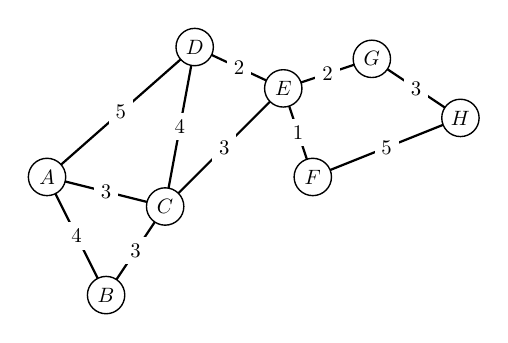
\begin{tikzpicture}[scale=0.75,transform shape]
  \SetVertexMath
  \Vertex[x=0,y=2]{A}
  \Vertex[x=1,y=0]{B}
  \Vertex[x=2,y=1.5]{C}
  \Vertex[x=2.5,y=4.2]{D}
  \Vertex[x=4,y=3.5]{E}
  \Vertex[x=4.5,y=2]{F}
  \Vertex[x=5.5,y=4]{G}
  \Vertex[x=7,y=3]{H}
  \Edge[label=$5$](A)(D)
  \Edge[label=$4$](A)(B)
  \Edge[label=$3$](A)(C)
  \Edge[label=$4$](D)(C)
  \Edge[label=$3$](C)(B)
  \Edge[label=$2$](D)(E)
  \Edge[label=$3$](C)(E)
  \Edge[label=$1$](E)(F)
  \Edge[label=$2$](E)(G)
  \Edge[label=$3$](G)(H)
  \Edge[label=$5$](F)(H)
\end{tikzpicture}
\centering
\caption{A graph representing the arrangement of student in the classroom.
Vertices represent students and edges represent opportunities to pass messages,
where the weight of an edge represents the likely hood the conversation
across the edge is compromised.}
\label{fig:class-graph}
\end{figure}

Recall that a graph is connected if there exists a path between every vertex
$u$ and $v$ in the graph.

\begin{defn}
Let $G = (V, E, w)$ be a graph. We call $G$ \emph{connected} if there is
a sequence of adjacent edges, i.e.~a path,  between every vertex $u$ and $v$
in $G$.
\end{defn}

Ideally, the students need to find a set of opportunities to pass messages,
$E' \subset E$, such that the total likely hood that any message is
compromised is as low as possible, and all of the students in the class
receive updates about the game.

\begin{defn}
Let $G = (V, E, w)$ be an connected, undirected, weighted graph such that
$w : E \to \mathbb{R}^+$. Then a \emph{spanning tree} $T$ of $G$ is defined as
a connected acyclic subgraph $T = (V, E', w)$, where $E' \subset E$.
\end{defn}

Formally, the students are looking for a spanning tree $T$ of $G$ where the
sum of the weights of the edges in the spanning tree are as low as possible
(or at least as low as that of any other spanning tree of $G$).

\begin{defn}
Let $T = (V, E', w)$ be a spanning tree of a graph $G$. Define the cost of the
spanning tree, $c(T)$ as
\begin{equation*}
    c(T) = \sum_{e \in E'}{w(e)}.
\end{equation*}
\end{defn}

Now, if a spanning tree $T$ of a graph $G$ has a cost at least as low as the
cost of every other possible spanning tree of $G$, we call $T$ a minimum
spanning tree of $G$.

\begin{defn} Let $T^*$ be a spanning tree of a graph $G$. We call $T^*$ a
\emph{minimum spanning tree} (MST) if
\begin{equation*}
    c(T^*) \leq c(T^)
\end{equation*}
for all alternate spanning trees $T$ of $G$.
\end{defn}

Given a minimum spanning tree, it is evident the students could achieve their
goal of communicating game updates to everyone while minimizing the likely hood
that any of their conversations are compromised. The broadcaster would simply
send his messages to students adjacent to him in the minimum spanning tree,
and these students would simply propagate their messages to their
neighbours on the spanning tree and so forth. Because the minimum spanning
tree represents a way of propagating the message with the lowest likely
hood that any conversation is compromised, and every student is part of the
minimum spanning tree, it is an optimal solution.

However, there still remains the problem of actually computing a minimum
spanning tree for their class. Assuming the students have an accurate idea of
the risk involved in speaking with any of their neighbours, and the teacher may,
at any moment, change their configuration of desks, how can the students
compute the minimum spanning tree for their class? Furthermore, how can they
be sure the spanning tree they compute is truly a \emph{minimum} spanning tree?

\section{Prim's Algorithm for Computing MSTs}

The following algorithm, due to Robert C. Prim, can be used to compute
the minimum spanning tree $T^*$ of a graph $G$.

\begin{defn}[{\bfseries Prim's Algorithm}] Let $G = (V, E, w)$ be an
connected, undirected, weighted graph such that $w : E \to \mathbb{R}^+$.
Then a minimum spanning tree $T^*$ of $G$ can be computed as follows:
\begin{enumerate}
    \item Begin with an empty set $T = \emptyset$ and a set $X
    = \left\{v\right\}$, where $v \in V$ is arbitrarily selected.
    \item Until $X = V$ repeat the step below.
    \item Let $Y$ be the set edges with one vertex in $X$ and the other
    vertex in $E - X$. Choose the edge $e \in Y$ with the smallest weight
    $w(e)$, breaking ties arbitrarily. Add $e$ to $T$ and add the vertex at
    the other end of $e$ to $X$.
    \item Output a minimum spanning tree $T^* = (V, T, w)$.
\end{enumerate}
\end{defn}

Intuitively, this algorithm corresponds to the following strategy for the
students:

\begin{enumerate}
    \item Begin with the broadcaster.
    \item Have the broadcaster pick a neighbour who, when spoken to, is least
    likely to compromise the pair. Pass messages to this neighbour.
    \item Now, with respect to the current group of people who know the news,
    pick a neighbour who, when spoken to, is least likely to compromise the
    group.
    \item Repeat the previous step until everyone in the class knows the latest
    information.
\end{enumerate}

Apart from their utility in colluding against teachers, minimum spanning
trees have a myriad of other important applications. They provide a solution
to a vast array of real world optimization problems, in fields as disparate
as computer networking to machine learning to infrastructure construction.
Therefore, it is important to know whether algorithms such as Prim's algorithm
really do work correctly to output minimum spanning trees.

The remainder of this paper is devoted to proving the correctness of
Prim's algorithm.

The proof of correctness will proceed in three parts. First, we show that the
algorithm terminates. Then we show that it outputs a spanning tree. Finally,
we that the output spanning tree is minimal.

\section{Connectedness and the Cut Lemma}

Before we begin, let us establish an important property of connected graphs,
which will allow us to more easily navigate the proofs ahead.

The motivation behind the following lemma is that it allows us to clearly
link what Prim's algorithm does at every iteration and the connectedness of its
input graph. Specifically, at every iteration, the algorithm adds an edge $e$
to $T$ with one endpoint in $X$ and another endpoint in $V - X$. If we can show
that for any choice of $X$ and $V - X$, this edge $e$ always exists, then
we can easily deduce many other properties of the algorithm.

\begin{lem}[{\bfseries The Cut Property}]
Let $G = (V, E, w)$ be a undirected, weighted graph. Then $G$ is connected
if and only if for any partition of $V$ into two sets $A$, $B$ such that
$A \cup B = V$ and $A \cap B = \emptyset$, there exists at least
one edge with a vertex in $A$ and a vertex in $B$, i.e., an edge which
crosses the cut $(A, B)$.

\begin{proof}
Assume $G$ is connected. Then there exists a path between every vertex $u$ and
$v$ in $V$. Let $A$ and $B$ be an arbitrary partition of $V$ such that
$A \cup B = V$ and $A \cap B = \emptyset$. Now suppose $a \in A$ and $b \in B$
are two vertices on different sides of the partition. Then by the connectedness
of $G$, there exists a sequence of edges between $a$ and $b$. Because $a$ and
$b$ are on different sides of the partition, there must be some edge $e \in E$
which has one endpoint in $A$ and the other endpoint in $B$. Hence, there
exists a cut which crosses $(A, B)$. Since $A$ and $B$ were chosen arbitrarily,
we've shown connectedness implies the cut property.

Now, assume that for all partitions $A$, $B$ of a graph $G$, and there
exists at least one edge $e \in E$ which has a vertex in $A$ and a vertex in
$B$. First, we show that for any choice of $A$ and $B$, $A$ and $B$ are
connected.

Suppose $A$ is not connected. Then there exist vertices $x_1, x_2, \ldots, x_k$
in $A$ which cannot be connected by a path. Let $X \subset A$ denote the
set of vertices which can be reached from $x_1$ by a path. Assume, without loss
of generality, that $B$ is connected, and the edge across $(A, B)$ has an
endpoint in $X$. Then for the partition $X \cup B$ and $A - (X \cup B)$ there
do not exist any edges which cross the cut $(X \cup B, A - (X \cup B))$, a
contradiction. Hence, $A$ must be connected. Similarly, $B$ must be connected.

Since $A$ and $B$ are connected by the edge $e$ and $A \cup B = V$, the entire
graph $G$ is connected. Therefore, we've shown the cut property implies
connectedness.
\end{proof}
\end{lem}

\section{Proof of Correctness of Prim's Algorithm}

Using the cut property, proving the correctness of Prim's algorithm becomes
much simpler. %More simple?%

\begin{thm}
Let $G = (V, E, w)$ be an connected, undirected, weighted graph. Then the
execution of Prim's algorithm for the input $G$ eventually terminates.

\begin{proof}
At each iteration of Prim's algorithm, an edge $e$ is added to $T$, with one
endpoint $u \in X$ and another endpoint $v \in V - X$. The endpoint $v$ is
then added to $X$. By the cut property, we know that such an edge exists for
all cuts across $(X, V - X)$. Therefore, at every iteration of the algorithm,
an endpoint $v \in V - X$ of an edge $e$ is added to $X$, and hence the order
of $X$ increases by $1$. Since the order of $X$ begins at $1$, and the order
of $V$ is finite, there must be an iteration at which $X = V$. Hence, Prim's
algorithm must terminate.
\end{proof}
\end{thm}

\begin{thm}
The output $T^* = (V, T, w)$ of Prim's algorithm constitutes a spanning tree
of the original graph $G = (V, E, w)$.

\begin{proof}
First, we show by induction that at every iteration of Prim's algorithm, the
output $T^*$ is connected.

In the base case, let $X = \left\{v\right\}$. Then by the cut property, we
know there exists an edge $e \in E$ across the cut $(X, V - X)$. Adding the
endpoint of $v'$ of $e$ to $X$ and the edge $e$ to $T$ clearly leaves $T^*$
connected as there is a path between all the vertices in $T^*$.

Now let us assume that $T^*$ is connected at some iteration $k$. We show that
$T^*$ is still connected at iteration $k + 1$.

By the cut property, we know that at any iteration of the algorithm, there
exists an edge $e$ across the cut $(X, V - X)$, where the endpoint of the cut
$v' \in V - X$ is not in $T^*$. Hence, assuming $T^*$ is connected, adding the
vertex $v'$ to $X$ and the edge $e$ to $T$ leaves $T^*$ connected. Therefore,
by induction, $T^*$ is connected when the algorithm terminates.

Next, we show that $T^*$ does not contain any cycles. By definition, Prim's
algorithm only adds an edge $e$ to $T$ when one vertex of the edge is in $X$
and the other is in $V - X$. The only way to create a cycle would be to add
an edge $e$ to $T$ with endpoints $x$ and $x'$ in $X$, when there already
exists a path between $x$ and $x'$. However, by definition, the algorithm
only adds edges with one endpoint in $X$ and the other in $V - X$. Therefore,
at every iteration, the algorithm will never add an edge $e$ to $T$ with
endpoints $x$ and $x'$ in $X$. Hence, at every iteration $T^* = (X, T, w)$
will be acyclic. Since the algorithm terminates when $X = V$, the output
graph $T^* = (V, T, w)$ will also be acyclic.

% Perhaps I should replace all of these ``will''s with ``must''s?

Now, since Prim's algorithm terminates when $X = V$, and the output
$T^* = (X, T, w)$ is connected and acylic, the output of Prim's algorithm
constitutes a spanning tree of the original graph $G$.
\end{proof}
\end{thm}

\begin{thm}
The output $T^* = (V, T, w)$ of Prim's algorithm constitutes a minimum spanning
tree of the original graph $G = (V, E, w)$.

\begin{proof}
First, we show by induction that at the end of every iteration of Prim's
algorithm, the algorithm's output $T^*$ is the minimum spanning tree of the
subgraph $H$ of $G$, where $H = (X, E', w)$ and $E' \subset E$, such that
$E' = \left\{\,e\in E\,|\:\text{the edge $e$ has both endpoints in}\:X\,
\right\}$.

% -- This seems way too complicated for a base case...

In the base case, let $X = \left\{v\right\}$, where $v$ is some arbitrary vertex in
$V$. By the cut property, we know that there exists at least one edge
across the partition $(X, V - X)$. Let $Y$ be the set of all edges across
$(X, V - X)$, and let $w(Y) = \left\{\,w(e_1), w(e_2), \ldots, w(e_k)\,\right\}$
be the set of weights of the edges in $Y$. By the well-ordering property
of the positive reals, there exists a set $Y'' \subseteq Y$ such that
the weight of all the elements in $Y''$ is at least as small as the weight
of any element in $Y$. Hence $Y'' = \left\{\,e \in Y\,|\, w(e) = k\,\right\}$,
where $k$ is the least element in $w(Y)$.

By definition, Prim's algorithm chooses arbitrarily among the edges if they
are all equally small. Since adding any of the edges in $Y''$ yields a
minimum spanning tree of $H$ with cost $c(T^*) = k$, the algorithm's output
$T^*$ will always be a minimum spanning tree of $H$.

Now, let us assume that Prim's algorithm outputs a minimum spanning tree of
the subgraph $H$ of $G$ at some iteration $k$. We show that at the end of the
next iteration $k + 1$, Prim's algorithm still outputs of minimum spanning tree
of $H$.

Once again, let $Y$ be the set of edges crossing the partition $(X, V - X)$,
and let $w(Y) = \left\{\,w(e_1), w(e_2), \ldots, w(e_k)\,\right\}$ be the set
of weights of the edges in $Y$. By the well-ordering property of the
positive reals, there exists a set $Y'' \subseteq Y$ such that the weight of
all the elements in $Y''$ is at least as small as the weight of any element
in $Y$. Hence $Y'' = \left\{\,e \in Y\,|\, w(e) = k\,\right\}$,
where $k$ is the least element in $w(Y)$.

Let the current cost of the spanning tree $T^*$ of $H$ be $c$. Adding any
edge $e \in Y''$ to the minimum spanning tree of $H$ yields a spanning tree
with cost $c(T^*) = c + k$. Therefore, no matter which edge $e \in Y''$ the
algorithm chooses, the output $T^*$ will always be a minimum spanning tree of
$H$.

Now, since the algorithm terminates when $X = V$, the set $E' = \left\{\,e\in E
\,|\:\text{the edge $e$ has both endpoints in}\:X\,\right\}$ will eventually
just be the set of edges in the original graph $G$. Hence, at the last
iteration, when $X = V$ and $E' = E$, the subgraph $H = (X, E', w)$ is equal to
$G = (V, E, w)$. And since the output of Prim's algorithm yields a
minimum spanning tree of $H$, it also yields a minimum spanning tree of $G$,
since $H = G$ at the last iteration.

Therefore, Prim's algorithm does indeed compute a mininmum spanning tree
$T^*$ of the inpute graph $G$.
\end{proof}
\end{thm}

Intuitively, the above theorem can be better understood if one realizes that
the set of minimum cost edges crossing the parition $(X, V-X)$ at the
$k$-th iteration will overlap considerably with the set of minimum cost edges
crossing the partition at the $k+1$-th iteration if there are a large number such edges
of minimum cost edges in the $k$-th iteration and the new edges crossing the
partition in the $k+1$-th iteration have cost less than the previous
minimum cost edges. In other words, Prim's algorithm will continue to add
minimum cost edges from previous iterations if they have lower cost. Thus,
choosing arbitrarily between edges is justified.

Another way to think about this is to imagine that we have a partition of
the graph, $(A, B)$, wherein $T_A$ and $T_B$ are the minimum spanning trees
of the subgraphs of $A$ and $B$ respectively. Now, no matter which minimum
cost edge crossing the partition we pick, the total cost will be the same.
Thus, we can break ties arbitrarily.

\section{Conclusion}

% Other algorithms for the MST, e.g. Kruskal's algorithm.}
%
% Where this fits into the general framework of greedy algorithms
% and combinatorial optimization.

\nocite{*}
\clearpage

\bibliographystyle{plain}
\bibliography{doc.bib}

\end{document}
